\section{Project Stage}
\subsection{System Architecture}

%\begin{figure}[H]
%	\centering
%	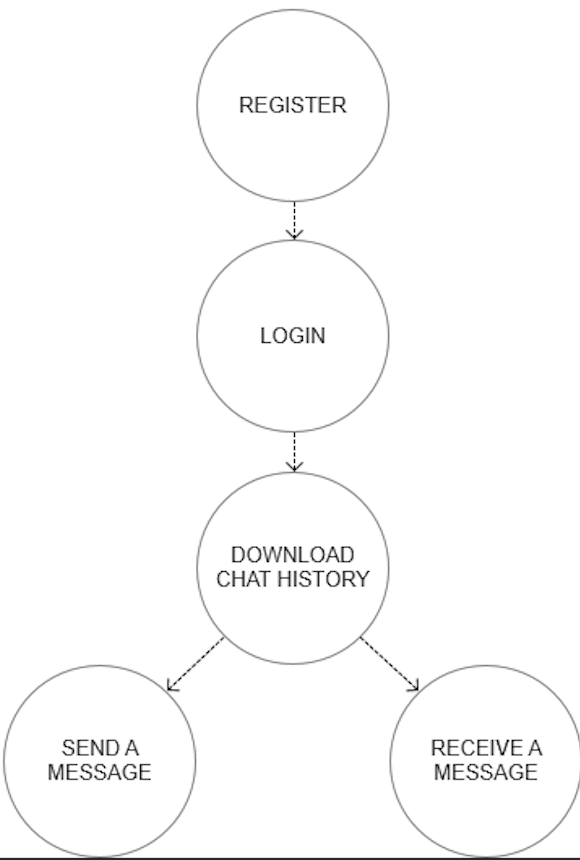
\includegraphics[width=\textwidth]{img/dag.png}  
%\end{figure}

\begin{figure}[H]
	\begin{subfigure}{\textwidth}
	\centering
		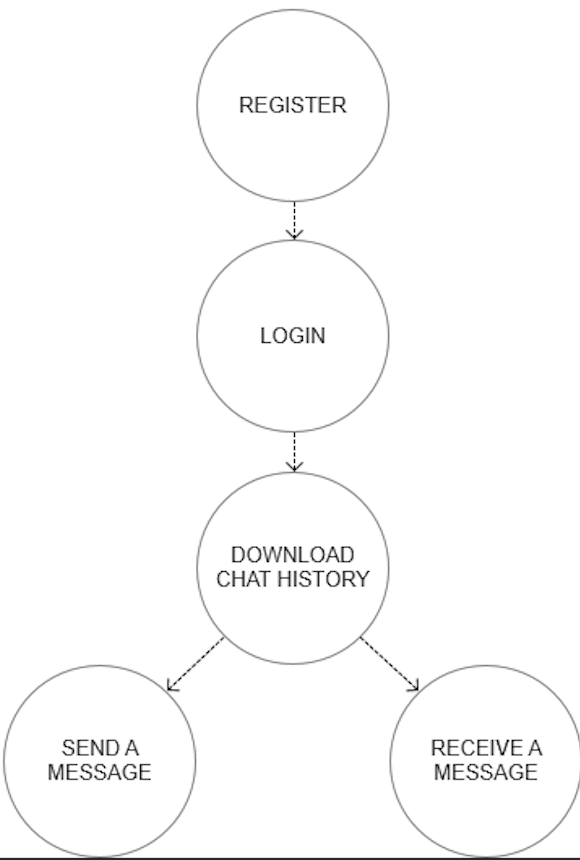
\includegraphics[width=0.3\linewidth]{img/dag.png} 
	\end{subfigure}
\end{figure}

As shown in the previous picture, the application is based on a client-server architecture, in which each client, in order to send a \textbf{message} to a \textbf{user}, contacts the main server which is in charge of determining receiver’s physical address and forward the \textbf{message} if it is online.
In the image some typical scenarios are represented to help better understand how \textit{Unisup} works. In particular:
\begin{enumerate}
	\item The message 1 $\xrightarrow{}$ A is sent from the client 1 destined to the client A:  it arrives at the main server that pushes it into the corresponding queue. The client A is online and there is no message to consume on the queue, so it is immediately forwarded.
	\item The message 2 $\xrightarrow{}$ A is sent from the client 2 destined to the client A:  as the previous one, it is pushed into A’s queue but this time the channel is busy. The message will be forwarded as soon as the channel comes idle again.
	\item The message 3 $\xrightarrow{}$ C is sent from client 3 destined to C: again, it is pushed on the correct queue. C is offline, so the message is not forwarded; it will be delivered as soon as C turns online again.
\end{enumerate}	
The OS picture inside clients means that the system works on every OS.
Eventually, the database icon has been added since it is required for mapping clients’ addresses and store chat histories. 


\subsection{Clients}
\subsubsection{Role of the Client}
During the normal usage of the application, the users interact with their client device, so the client is the principal actor of our application.
As described in the use cases analysis user i can register to the application, sign in into his/her account, then he/she can do all the operation of a typical instant-message application like sending/receiving messages and read old messages through clicking on chats. Because the applicative isn’t bound to a specific client, as \textit{Whatsapp} is, a client device can be used by multiple \textbf{users}, they only need to register/login to their account.
From an architectural point of view, the \textbf{client} is only in charge of providing the \textbf{user} a GUI and the communication with the server. The \textbf{client}  device does not store the history of the messages, nor information about the user, but it is in charge of showing chats and messages in the correct natural order that is sorted by ascending timestamp. On client-side, a multithreaded approach has been developed according to the following DAG.

Since SEND A MESSAGE and RECEIVE A MESSAGE are concurrent actions, they are performed by different flows of execution. The only shared data structured is the message list of the relative chat, so the access to it must be synchronized.

\subsubsection{Technologies}
The applicative code runs entirely on the clients: every interaction with the GUI is handled locally and may trigger a send request to the server. The principles technologies used in the client side are JavaFX and Jinterface.
\begin{itemize}
	\item The GUI is implemented using JavaFX classes, some of them were extended for creating ad-hoc classes that can be found in the javafxexstension package. The use of JavaFX is due to make the application more user-friendly.
	\item The Jinterface package provides a set of tools for communication with Erlang processes. In this way the client can send and receive messages to the server, define receive mailboxes and so on.
\end{itemize}

\subsection{The Server}
\subsubsection{Role of the Server}
The server is the core of our system, every client has to communicate with it in order to accomplish any operation of that one’s listed in chapter 2.1.
The server is in charge of:

\begin{itemize}
	\item Register user data at registration time, remembering username and password.
	\item Login users by checking username and password, binding usernames with the physical client process in charge of the receiving of the message.
	\item Forward any message to the correct client: every sender client contacts firstly the server (so that clients are not requested to store physical addresses of other clients, they specify WHAT and not HOW to deliver messages). The server is capable, having as input a username, of determining the relative physical address and forward the message.
	\item Register every in-transit message in order to permit the restoring of the chat list for every client
	\item Queuing correctly the messages that are destined to the same client, so that to handle concurrency and buffering of messages whose receiver is offline. 
\end{itemize}

\subsubsection{Implementation of the Server}
In order to achieve a high-performance application, it is crucial to have a lightweight \textbf{server} code, capable of handling quickly every request and of parallelizing work when possible. As discussed in the paragraph 3.2.1, concurrent actions inside a \textbf{client} are handled by the \textbf{client} itself; the \textbf{server}  is in charge of handling concurrency between different \textbf{clients}. In order to accomplish these requirements, we chose to implement the server entirely in Erlang, so that:
\begin{itemize}
	\item The lightweight of the language is particularly suitable to ensure high performance on the simple actions that the server must perform
	\item The Mnesia persistent support guarantees fast operations and internal handling of concurrent accesses to the data (see par. 3.3.3)
	\item The RabbitMq library queues messages destined to every client with a FIFO policy. It ensures correct concurrency handling and buffering of messages whose receiver is offline.
\end{itemize}
In addition, to improve performance and abstract the \textbf{server} structure, we decided to adopt the \textit{Gen\_Server} behavior to handle \textbf{client} requests.
Moreover, to decrease the coupling between \textbf{client} and the \textbf{server}, a listener module has been provided. At each request it spawns a process that prepares data structures, forward the request to the \textit{Gen\_Server}  after a preliminary pattern matching and finally changes the format of the response in a \textit{client-side-easy-to-parse} way. 


\subsubsection{Persistent Data Storing}
For storing all the information regarding the users and their relative messages we make use of Mnesia. The choice to use Mnesia is driven by the fact that Mnesia is designed with requirements like the following:
\begin{itemize}
	\item Fast real-time key/value lookup
	\item Complicate non-real-time queries mainly for operation and maintenance
	\item High fault tolerance
\end{itemize}
Mnesia is also interesting because of its tight coupling to Erlang, thus almost turning Erlang into a database programming language. This has many benefits, the foremost is that the impedance mismatch between the data format used by the DBMS and the data format used by the programming language, which is used to manipulate the data, completely disappears.

\textit{UniSup} stores the information cited above in two tables named \textit{unisup\_users} and \textit{unisup\_messages} in records made in this way, respectively:
\begin{lstlisting}[language=erlang]
	-record(unisup_messages, {sender,
               receiver,
               text,
               timestamp
              }).

	-record(unisup_users, {username,
                  password,
                  nodeName,
                  pid
                }).
\end{lstlisting}

Because we want to keep the data in a persistent way, so even there is a crash in our server the records shouldn't be lost, the tables are saved using the \textit{disc\_copies} option, thus we maintain the records store in memory and on the disc. Every time the server starts \textit{Mnesia} it waits if the table are present:

\begin{lstlisting}[language=erlang]
mnesia:create_schema([node()]),
  mnesia:start(),
  case mnesia:wait_for_tables([unisup_messages, unisup_users], 5000) == ok of
    true ->
      ok;
    false ->
      mnesia:create_table(unisup_users,
        [{attributes, record_info(fields, unisup_users)},
          {disc_copies, [node()]}
        ]),
      mnesia:create_table(unisup_messages,
        [{attributes, record_info(fields, unisup_messages)},
          {type, bag},
          {disc_copies, [node()]}
        ])
  end
\end{lstlisting}
If they are then we simply load them, otherwise we create the tables again.
Another important thing is that we store the record in \textit{unisup\_messages}  using the \textit{bag type}. A \textit{bag} table can have multiple entries with the same key, as long as the tuples themselves are different. This means that the table can contain \textit{\{sender, receiver, text, timestamp\}} and \textit{\{sender, receiver, text, timestamp2\}} without any problem. which would be impossible with \textit{set} tables (they have the same key). However, we couldn't have \textit{\{sender, receiver, text, timestamp\}} twice in the table, but that is impossible because the timestamp will surely be different. 

\subsubsection{Queueing}
To provide the common messaging behavior for our application, we considered using queuing system by exploiting \textit{RabbitMQ}. Each user must have a queue for receiving the messages. Explicitly, each \textbf{user}  is a consumer, and consumes messages from the queue corresponding to his/her username. In this way, we can also manage the synchronization issue related receive a message. The first message comes into the \textit{queues} will be consumed and delivered to the user first, so we have FIFO queues. Since all the communication pass through the server in our application, we need to send the request for consuming to the server when a user gets online. Accordingly, when a user sends a message to another one, the message should be sent to the server and then the server passes it to the receiver queue. Finally, the \textit{queues} must be persistent since we do not want to the not consumed messages when the connection between server and \textit{RabbitMQ} goes down. 
In the following example, user A (Sender) sends a message to \textbf{user} B (Receiver). \textbf{User}  A does not care if the B is online or not.  Request for Consuming will be sent to the server automatically after the B gets online. 

\begin{figure}[H]
	\centering
	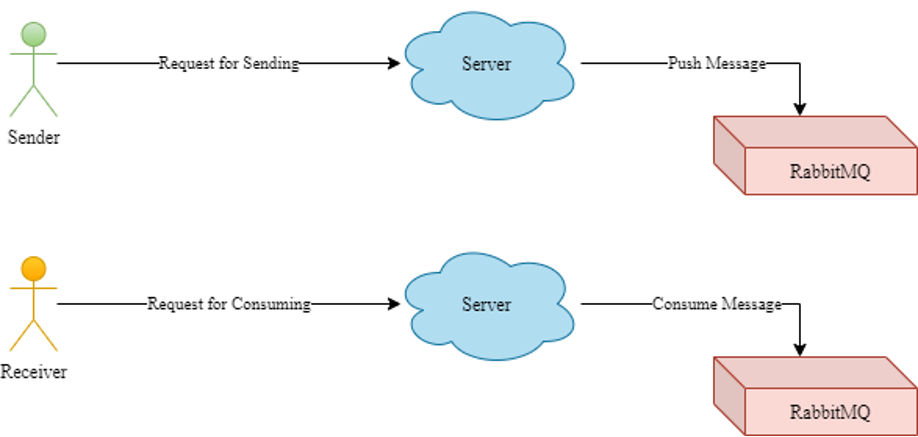
\includegraphics[width=\textwidth]{img/rabbitMQ.png}  
\end{figure}

\subsubsection{Queueing Architecture}
We used direct exchange of \textit{RabbitMQ} , since our messaging system only contains one to one communication, so we do not consider the possibility of creating channels or groups.
We run a process to handle each user request (sending or consuming). This process adopts \textit{gen\_server} behavior to provide several functionalities to the application. After the initialization, the process would react to one of the following commands:

\begin{enumerate}
	\item \textbf{Reset}: The process will be restarted and re-initialized. 
	\item \textbf{Stop}: The process will be killed, so no more request will be handled. We use this command when stopping the whole server application. 
	\item \textbf{Push}: The input message will be converted to dictionary of binary entries and encoded. Then it will be sent to the receiver queue. If the push was successful, pushed atom will be returned. 
	\item \textbf{Delete User}: The queue of the user will be deleted. 
	\item \textbf{Request Consuming}: When a user sends this request, we must dedicate a channel and consuming process to the user. The channel is required for communication between the consuming process and RabbitMQ, because it connects to the specified queue. The consuming process receives any message from the channel. Then the incoming message will be sent to the user (Receiver) process id.
	\item \textbf{Terminate Consuming}: When the user logouts, we must close its channel. Otherwise, the opening channels may cause the overhead in our server.
\end{enumerate}

In addition, after a certain amount of time (in our case it is thirty minutes), we refreshed the channels by deleting and creating another one. In practice, the heartbeat connection between  \textit{RabbitMQ}  and the server will determine to close the connection after not receiving any data for a certain period. Therefore, we must also check if the connection is dead, recreate the connection and channel again. 

\subsection{Synchronization Management}
In this chapter, we discuss the main synchronization problems that arise from our application, discussing and motivating the solutions we adopted to address concurrency.
As we will explain in the next paragraphs, the general approach we chose is the usage of frameworks and other tools that provide efficient and automatic concurrency handling, instead of \textit{“reinventing wheel”}. When this approach was not possible or not so convenient, we addressed concurrency issues manually, always separating tasks from execution strategies. 

\subsubsection{Client-Side}
Every client can serve only a user at the time, so there is no need of concurrency between different users. However, different tasks on the same client are executed by different threads, and in particular:
\begin{itemize}
	\item The main thread, it only spawns the next thread
	\item \textit{JavaFX Application thread} is in charge of listening for events and performing the actions specified by the relative controller. When an event occurs, this thread performs controller’s code, which means that it may send messages to the server, update the model and/or update the view. After the login is correctly performed by this thread, the next one is spawned: it will be interrupted when a new logout request is performed.
	\item A listener thread repeatedly blocks itself waiting for a message to come. Every 5 seconds, if no message has been sent, it wakes up checking if it has received interruption request. If not, it blocks itself again. When a new message arrives, it updates the model and sends a request to the view for the update, then another iteration is performed. The relative pseudo-code is the following:
\end{itemize}

\begin{lstlisting}[language=java]
while(true):
	do:
		M=receiveMessage(TIMEOUT);
		If(interruptRequestReceived()):
			Terminate;
		endif
	while(M==null);
	updateModel(m);
	requestForGuiUpdate(m);
endloop
\end{lstlisting}
Since both the  \textit{JavaFX Application thread} and the \textit{listener thread} can access the model and the \textbf{GUI}, a synchronization mechanism is required. On the other hand, the two threads contact the server through different mailboxes, so no sync is required at communication level (all the common data structures are final).
For what concerns the model, it is pointless to make all the data structures synchronized, indeed:

\begin{outline}
	\1 The write accesses to a \textbf{Message} are only made at construction time, thus only read accesses are allowed.
	\1 The Chat’s \textit{usernameContact} field is final. On the contrary the message list (history) and the number of the \textbf{unread messages} can be accessed by both the threads: these fields are atomic (\textit{java.util.concurrent.atomic}). The accesses to the list are always read or append, so no risk of update while we iterate it.
	\1 The \textbf{User}’s account fields are unique for the session lifecycle: they are only updated at login time, when the listener thread does not exist yet. Anyway, the list of chat is again shared by the threads (\textit{synchronizedList} has been exploited).
This time, it could also be accessed in write mode by the listener while the other thread is iterating it. In order to prevent this, we lock it while the iteration is performed. Why this choice instead of a thread-safe iterator?
	\2 Because for our application purposes, we expect to have a small amount of contacts, thus the iteration will be fast
	\2 Because we only have 2 threads, so there is a very little chance of concurrent accesses
	\2 Because the operations performed at each iteration and the ones performed while we access it in write mode are very easy, which reduces the amount of time the data structure is locked
	\1 For these reasons, we decided not to use a safe iterator, which could have introduced a higher amount of overhead, choosing a normal synchronized-block approach instead.
\end{outline}
A totally different speech has to be made for addressing \textbf{GUI concurrency}. In order to explain it, we must take into account how \textit{JavaFX} works.
The Application Thread is in charge of executing the controller code corresponding to every event has been fired: when an event is triggered, it is inserted into a  \textit{JavaFX} queue; the \textit{Application Thread} loops the queue executing the code associated to each event. When the queue is empty, the  \textit{Application Thread} is blocked.
\textit{JavaFX} \textbf{does not allow user-defined threads to update the visualization}, so there is no need to synchronize GUI data structures since the listener thread cannot access them.
But how do we update the visualization when a message arrives?
The \textit{JavaFX} concurrency API allows to define a \textit{Worker} (for example, a Task), but it is spawned only when an event is triggered: it is not suitable for our application, in which we want that receive messages are shown asynchronously \textit{w.r.t.} the user interaction with the GUI. Note that although the listener blocks itself waiting for a message, from the global point of view we can see this receive operation as asynchronous: even if a new message does not arrive, the application is still responsive to user inputs.
The approach we choose is exploiting the \textit{javafx.application.Platform.runLater()}s method, that allows to push a new Runnable into the \textit{Application Thread} queue. 
Of course we took care not to insert code that accesses the model in this \textit{Runnable} object.

\subsubsection{Server-Side}
For what concerns the server, the handling of requests coming from different users requires a fine grain level of concurrency and parallelism. Indeed, in order to ensure high performance, we wanted the server to be able to handle multiple request at a time: the need for a quick and lightweight server and for a developer-friendly handling of the concurrency guided us to the choice of implementing it completely in \textit{Erlang}. In fact:

\begin{itemize}
	\item \textit{Erlang}’s processes share no memory (actor model inspired), so we can spawn a process for each request with no concern about possible concurrent accesses to server’s data structure
	\item \textit{Erlang}’s communication protocol hides the details of the physical network layer: it was a very helpful starting point to develop an application capable of hiding also client-server communication, so that sender and receiver seem to be directly connected each other
	\item \textit{Erlang} code is fast to run, so it can ensure good performances even if we have to handle a discrete number of processes
\end{itemize}
The \textbf{server} is basically \textit{service-oriented} and \textit{not resource-oriented}, which means that it does not provide documents or files to the clients, nor it computes and send back results. \textit{Unisup} server is basically a middleware component that ensure communication between end users (hiding IDs of processes and the reliable data transfer protocol) and persistence to their messages, so that a user can access \textit{Unisup} from any \textbf{client} and always be able to get his/her own chat history and communicate with his/her contacts.
For these reasons, all we needed in our server is:

\begin{itemize}
	\item A \textbf{listener module}, which is in charge of listening for \textbf{client} request and spawning a process to handle the request. This module, when initialized, sets up also the main server data structure (\textit{Mnesia persistency} and \textit{RabbitMQ queueing}). The listener is an always-up registered process, so that clients have not to deal with PIDs. The listener is able to filter out messages whose syntax is not the one established for every \textit{Unisup} message (\textit{SenderPid, OpIdAtom, Arguments})
	\item A \textbf{request handling module} (\textit{callback}) built on the top of the \textit{gen\_server} behavior (which provides a standard API and efficient communication operations). This module, together with the filtering of all the messages whose couple (\textit{OpIdAtom, Arguments}) is not recognized as valid, is the one that processes requests communicating with \textit{Mnesia} and/or \textit{RabbitMQ} if required and sending back a message that, depending on the specific request, can be an \textit{ACK/NACK}, a true/false result or more complex results (\textit{e.g.}, chat history, \textit{i.e.} a list of messages)
	\item A \textit{Mnesia} module with all the functions that a \textbf{client}  could request to run on the shared database. Only the callback module is able to call these functions
	\item A \textit{RabbitMQ} module with all the functions for the handling of the queues. Only the callback module is able to call these functions
	\item Utility modules. They contain no shared data structures, so no need for synchronization.
\end{itemize}

Analyzing these modules, it’s easy to see that, in spite the fact that we handle multiple processes together, thanks to \textit{Erlang} and the other frameworks’ properties, we don’t need to address concurrency manually, indeed:

\begin{itemize}
	\item The \textit{listener module} processes a message at a time.
	\item The \textit{multiple processes} spawned by the listener execute the callback code. Anyway, thanks to the \textit{Erlang}’s lack of state and absence of shared memory, each request is independent from the others
	\item The \textit{Mnesia Database} is a shared data store. In order to guarantee mutex accesses to the data, we chose to operate on it through \textbf{Mnesia transactions}, \textit{i.e.}, \textit{ACID operations} capable of ensuring \textbf{Atomic} and \textbf{Isolated statements}. Thanks to transactions, there is no risk for critical races on the data between processes.
	\item The \textit{RabbitMQ} module provides by construction concurrency management: push and consume are primitive operations (at this level of abstraction of course), so there is no possibility of critical races between processes. 
The queueing management also prevents the uncontrolled growth of needed channels in case of high amount of traffic, and can handle messages destined to offline users
\end{itemize}

\subsection{Rebar3}
Since our server is implemented in erlang, we realized that we can use Rebar3 to manage our application in proper way. Rebar3 is a build tool and package management for creating and deploying erlang applications [1 – 2]. To use \textbf{amqp} (\textit{RabbitMQ}) and \textbf{jsx} (\textit{JSON}) libraries, we added the dependencies in \textit{Rebar3 config file}, so all of them work under a unified project. To compile and run our server application we simply run the following command

\begin{lstlisting}[language=python]
	$ rebar3 shell --name unisup_server@localhost --setcookie unisup --script src/run\_listener.escript
\end{lstlisting}

